% Diagram for the Bernoulli Principle
% Author: Roland Puntaier
\documentclass[tikz,border=10pt]{standalone}
\usetikzlibrary{calc}
\begin{document}
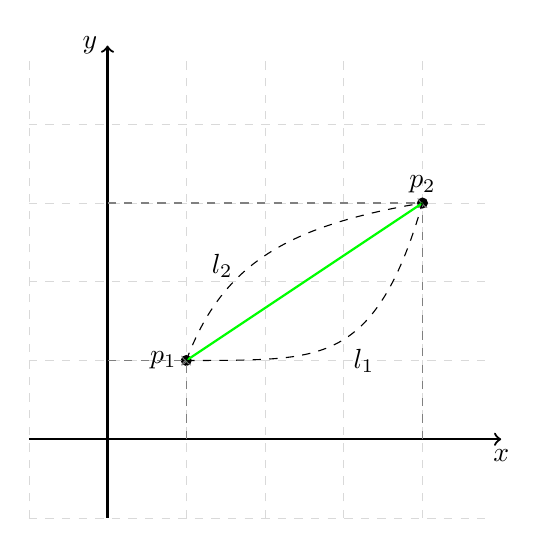
\begin{tikzpicture}

% Grid
\draw[help lines, color=gray!30, dashed] (-1,-1) grid (4.9,4.9);

% Axis
\draw[->,thick] (-1,0)--(5,0) node[below]{${x}$};
\draw[->,thick] (0,-1)--(0,5) node[left]{$y$};

% Points
\fill (1,1) circle[radius=2pt] node[left]{$p_1$};
\fill (4,3) circle[radius=2pt] node[above]{$p_2$};

% Dashed coords

%% p1
\draw[->,color=gray,dashed] (1,0)--(1,1);
\draw[->,color=gray,dashed] (0,1)--(1,1);

%% p1
\draw[->,color=gray,dashed] (4,0)--(4,3);
\draw[->,color=gray,dashed] (0,3)--(4,3);

% Straight line

\draw[-,color=green,thick] (1,1)--(4,3);

% Curve line 1
\draw[black,dashed] 
    plot[domain=1:4, samples=100] (\x, { \x ^ 7 / 8191.5 + 1 }) 
    node[right] at (3,1) {$l_1$};

% Curve line 2
\draw[black,dashed] 
    plot[domain=1:4, samples=100] (\x, { - 8 / 3 / \x + 11 / 3 }) 
    node[right] at (1.2,2.2) {$l_2$};

\end{tikzpicture}
\end{document}
